\documentclass[UTF8]{ctexart}
\usepackage{mathtools,wallpaper}

\usepackage{t1enc}
\usepackage{pagecolor}
\usepackage{geometry}
\usepackage{diagbox}
\usepackage{graphicx}
\usepackage{wrapfig}
\usepackage{amssymb}

\geometry{left=2cm,right=2cm}

\begin{document}

\CTEXsetup[format={\Large\bfseries}]{section}
\title{实验报告}  
\author{徐亦昶 PB20000156}
\maketitle
\section{实验题目}RGB配色实验
\section{实验目的}
\begin{enumerate}
    \item 了解色度学相关知识
    \item 理解LED发光原理和基本特性
    \item 掌握色光相加混合规律
\end{enumerate}
\section{实验原理}
自然界中人眼所能见到的大多数颜色是由红、绿、蓝三种相互独立的基色混合而成的。这三种基色的比例决定混合后所得颜色的色调和色饱和度。本实验中,要用到如下合成法则:
\begin{enumerate}
    \item 红色+绿色=黄色
    \item 绿色+蓝色=青色
    \item 蓝色+红色=紫色
    \item 红色+绿色+蓝色=紫色
\end{enumerate} 
发光二极管的核心是PN结。它具有一般 PN 结的特性,即正向导通,反向截止、击穿。在正向电压下,电子由N区注入P区,空穴由P区注入N区,
这些电子与空穴结区发生复合后会发射光子。发光中心波长$\lambda$和禁带宽度$E_g$的关系如下:
\[\lambda=\frac{1240}{E_g}\left( nm \right),\]
其中$E_g$的单位为电子伏特,可通过I-U图上导通电压对应切线与U轴的交点得到。
\section{实验内容}
\subsection{LED的伏安特性测量}
如图接线,调整电流I至5mA,10mA,...,100mA,分别测量对应的电压表示数U(V),并绘制I-U特性曲线。
\begin{figure}[h]
    \centering
    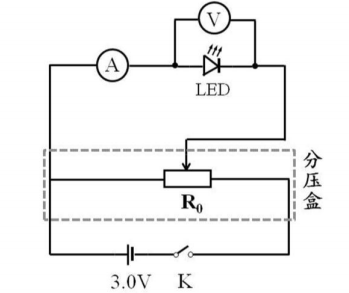
\includegraphics[scale=1]{伏安特性.PNG}
    \caption{LED的伏安特性测量电路图}
\end{figure}
\subsection{LED的发光波长测量}
\begin{enumerate}
    \item 做伏安特性曲线的渐近线,设与U轴交于$U_0$,进而得到$E_g$。
    \item 由$\lambda=\frac{1240}{E_g}$算出红、绿、蓝LED的发光中心波长。
\end{enumerate}
\subsection{LED的光强与电流关系}
\begin{enumerate}
    \item 如图安装仪器,其中LED灯与光电池之间的距离为20cm。
    \item 断开LED灯,测出电压表示数U(V)作为背景光强。
    \item 调整LED亮度,进而将电流I调整至5mA,10mA,...,100mA,分别测量对应的电压表示数U(V)作为LED的相对光强。
    \item 绘制绿色LED的L-I特性曲线,给出近似函数关系。
\end{enumerate}
\begin{figure}[h]
    \centering
    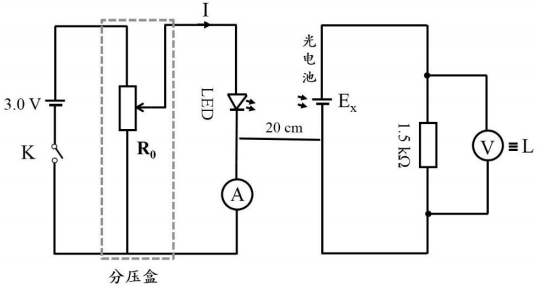
\includegraphics[scale=1]{光强与电流关系.PNG}
    \caption{LED的光强与电流关系电路图}
\end{figure}
\subsection{加法混合实验}
\begin{enumerate}
    \item 如图所示配置电路,同上一个实验测出背景光强。
    \item 用两个LED在白屏上配出标准色卡的黄色、青色、紫色(在这里边需要调整白屏的位置,使得LED光斑在白屏上呈现同心圆)。
    \item 将光电池放置于白屏处,分别测量
    \item 使用三个配标准比色卡的白色,类似地测出三个LED的及配色的相对光强,给出三个基色的光强比。
\end{enumerate}
\begin{figure}[h]
    \centering
    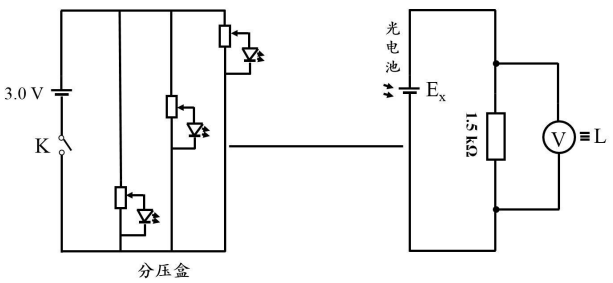
\includegraphics[scale=1]{相对光强.PNG}
    \caption{加法混合实验电路图}
\end{figure}
\newpage
\section{数据记录}
\begin{table*}[htbp]
    \centering
    \fontsize{8}{10}\selectfont
    \caption{LED的伏安特性测量}
    \scalebox{1.2}{
    \begin{tabular}{|c|c|c|c|c|c|c|c|c|c|c|}
    \hline
    \diagbox{LED\\种类}{电流I\\(mA)}& 5.0 & 10.0 & 15.0 & 20.0 & 25.0 & 30.0 & 35.0 & 40.0 & 45.0 &50.0 \\
    \hline
     红&1.7594&1.7912&1.8126&1.8284&1.8442&1.8627&1.8707&1.8833&1.8951&1.9067\\
     \hline
     绿&2.212&2.258&2.291&2.314&2.337&2.357&2.375&2.393&2.411&2.427\\
     \hline
     蓝&2.534&2.567&2.588&2.604&2.621&2.635&2.647&2.661&2.673&2.683\\
     \hline
    \end{tabular}}
\end{table*}
\begin{table*}[htbp]
    \centering
    \fontsize{8}{10}\selectfont
    \caption{LED的伏安特性测量(续表)}
    \scalebox{1.2}{
    \begin{tabular}{|c|c|c|c|c|c|c|c|c|c|c|}
    \hline
    \diagbox{LED\\种类}{电流\\I(mA)}& 55.0 & 60.0 & 65.0 & 70.0 & 75.0 & 80.0 & 85.0 & 90.0 & 95.0 & 100.0 \\
    \hline
     红&1.9186&1.9293&1.9390&1.9489&1.9567&1.9693&1.9778&1.9884&1.9957&2.004\\
     \hline
     绿&2.441&2.454&2.469&2.483&2.498&2.511&2.522&2.533&2.546&2.554\\
     \hline
     蓝&2.696&2.705&2.715&2.728&2.738&2.747&2.756&2.765&2.775&2.783\\
     \hline
    \end{tabular}}
\end{table*}
\begin{table*}[htbp]
    \centering
    \fontsize{8}{10}\selectfont
    \caption{LED的光强与电流关系(未减去背景光强)}
    \scalebox{1.3}{
    \begin{tabular}{|c|c|c|c|c|c|c|c|c|c|c|}
    \hline
    电流I(mA)& 5.0 & 10.0 & 15.0 & 20.0 & 25.0 & 30.0 & 35.0 & 40.0 & 45.0 &50.0 \\
    \hline
    光强L(V)&0.0024&0.0051&0.0081&0.0111&0.0141&0.0171&0.0198&0.0230&0.0261&0.0290 \\
    \hline
    \end{tabular}}
\end{table*}
\begin{table*}[htbp]
    \centering
    \fontsize{8}{10}\selectfont
    \caption{LED的光强与电流关系(续表)}
    \scalebox{1.3}{
    \begin{tabular}{|c|c|c|c|c|c|c|c|c|c|c|}
    \hline
    电流I(mA)& 55.0 & 60.0 & 65.0 & 70.0 & 75.0 & 80.0 & 85.0 & 90.0 & 95.0 & 100.0\\
    \hline
    光强L(V)&0.0317&0.0347&0.0376&0.0408&0.0434&0.0465&0.0493&0.0522&0.0550&0.0580  \\
    \hline
    \end{tabular}}
\end{table*}
\begin{table*}[htbp]
    \centering
    \fontsize{8}{10}\selectfont
    \caption{LED的光强与电流关系(已扣除背景光强)}
    \scalebox{2}{
    \begin{tabular}{|c|c|c|c|c|}
    \hline
    配色& 黄色 & 青色 & 紫色 & 白色\\
    \hline
     红色相对光强(V)&0.1190&\diagbox{}{}&0.0478&0.0654\\
     \hline
     绿色相对光强(V)&0.0245&0.0149&\diagbox{}{}&0.3076\\
     \hline
     蓝色相对光强(V)&\diagbox{}{}&0.0393&0.0826&0.0025\\
     \hline
     配色相对光强(V)&0.1422&0.0540&0.1283&0.4207\\
     \hline
     基色光强比(V)&4.86&0.38&0.58&1.00:4.70:0.04\\
     \hline
    \end{tabular}}
\end{table*}
\newpage
后两个实验中,背景光强均为0.0002V。
\section{数据计算}
\subsection{LED的伏安特性测量}
利用人工神经网络(sigmoid为激活函数,1*5*10*1,包含两个隐藏层)拟合伏安特性曲线如图:
\begin{figure}[h]
    \centering
    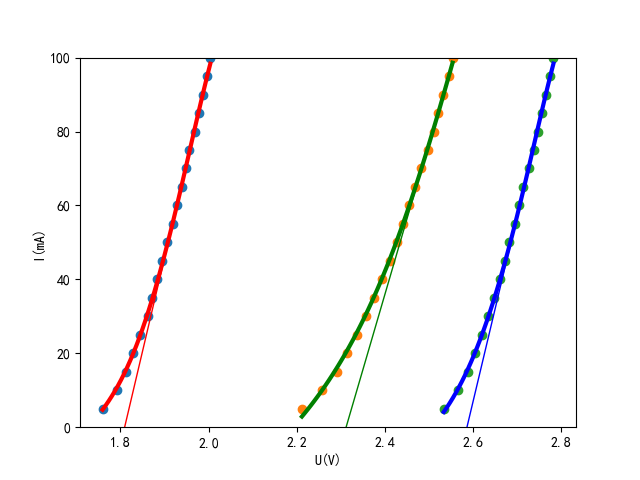
\includegraphics[scale=1]{伏安特性曲线.png}
    \caption{伏安特性曲线}
\end{figure}
\newline
其中切线与x轴的截距$U_0$分别为:1.810(红)、2.312(绿)、2.587(蓝)。
\subsection{LED的发光波长测量}
由上可知红、绿、蓝LED的$E_g$分别为1.810,2.312,2.587。
从而$\lambda$分别是685nm,536nm,479nm。
\subsection{LED的光强与电流关系}
容易发现两变量呈线性关系,因此做线性拟合。
\begin{figure}[h]
    \centering
    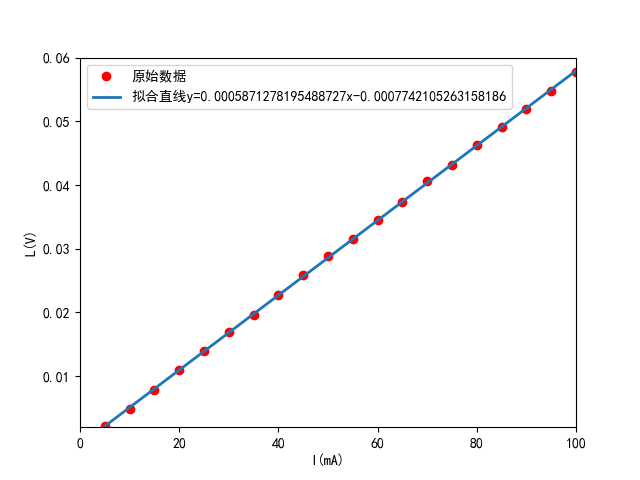
\includegraphics[scale=1]{光强与电流关系拟合.PNG}
    \caption{LED的光强与电流关系(已扣除背景光强)}
\end{figure}
直线方程:L=0.0006I-0.0008.
\newpage
\section{不确定度分析}
\subsection{LED的伏安特性测量}
在曲线的拟合中,使用方均根作为神经网络的损失函数值,loss(红)=0.052,loss(绿)=0.053,loss(蓝)=0.045。
\subsection{LED的光强与电流关系}
使用origin可算出直线斜率和截距的标准差分别是0.0000012,0.0000671,相关系数是0.99997。
对于斜率:
\[u_A=\frac{0.0000012}{\sqrt{20}}=2.68\times 10^{-7}\]
\[t_{0.99}=2.86\]
\[\therefore u_t=t_{0.99}u_A=7.66*10^{-7}\]
对于截距:
\[u_A=\frac{0.0000671}{\sqrt{20}}=1.5\times 10^{-5}\]
\[t_{0.99}=2.86\]
\[\therefore u_t=t_{0.99}u_A=4.29\times 10^{-5}\]
\section{思考}
\begin{enumerate}
    \item 人眼的视敏特性是指人眼对不同波长的光具有不同的灵敏度的特性叫视敏特性。视敏特性常用视敏函数来表示。
    \item 亮度不同,乙是甲的两倍。
    \item 色光混合:红+绿=黄,绿+蓝=青,蓝+红=紫,红+绿+蓝=白;色料
    混合:红+黄=橙,红+蓝=紫,蓝+黄=绿,红+黄+蓝=黑。色料三原色红、黄、蓝的补色绿、紫、橙。
\end{enumerate}

\end{document}